%%%%%%%%%%%%%%%%%%%%%%%%%%%%%%%%%%%%
%%%%%%%%%%%%%%%%%%%%%%%%%%%%%%%%%%%%
%%%%%%%%%%%%%%%%%%%%%%%%%%%%%%%%%%%%
\subsection{Relational and semistructured operations}\label{ssec:gsmrelop}
 The previous subsection discussed the definition of set (and object) operators on top of GSQL. \marginnote{$\lhd$ \textit{Attribute labelled Set operators over relations' GSM representations.}} For this reason, we must make sure that the former definitions are also compliant with GSM translations of relations as defined in Algorithm \vref{alg:reltonested}: given that the aforementioned translation maps each possible relation into one object $r_o$ associating all the tuples $t_i$ via a single \ONTA attribute ($t_i\in \phi(r_o,\ONTA)$), by definition of the former operators we have that the desired set operation will be actually performed over the set of objects defined over \ONTA. Therefore, the former section provides a straightforward definition for set operations that are compliant with objects produced by a translation from the relational model, and hence they do also implement set operations for the relational model. Moreover, the union actually defines an outer union \cite{deII}, where the resulting relation has the resulting schema which is the union of  two relations' schemas.

Similar considerations can be also performed for the relational filtering (also known as selection, $\sigma$) operator: if we restrict the filtering property just to the elements contained by the object reference in \ONTA, we can express the $\sigma_P$ operator from $\texttt{filter}_P$ presented in Equation \vref{eq:selection} as follows:
\[\texttt{filter}_{\scriptline{t -> \{not (t in (g.phi[}\ONTA\texttt{])) {\color{RoyalBlue}||} } P\texttt{(t)\}}}(n)\]
Please note that such restriction may be completely ignored for semistructured models, where the \texttt{filter} operator may be directly introduced.


At this point, we want to show that the $\texttt{map}$ operator can express other algebraic operators that have  already been defined in current literature, such as  embedding ($\varepsilon_{EF}$) and the projection ($\pi_{PF}$) operators presented in \cite{Magnani06}. Both operations acts as a specific instance of map operators: while $EF$ is defined as a function extending the object's collection with new identifiers or creating new associated collections, $PF$ either reduces the number of collections or reduces their content. Consequently, both operators can be defined as follows:

\begin{definition}[Embedding]
	Given a GSM $n$, its \textbf{embedding}\index{GSQL!$\varepsilon$} is defined as a specific map function $EF$ such that $\forall o\in O.\forall p\in\lang. EF(o,p)\supseteq \phi(o,p)$:
	\[\varepsilon_{EF}(n)=\texttt{map}_{\ell_{nn'},\xi_{nn'},\phi_{nn'}\oplus EF}(n)\]
\end{definition}

\begin{definition}[Projection]
	Given a GSM $n$, its \textbf{projection}\index{GSQL!$\pi$} is defined as a specific map function $PF$ such that $\forall o\in O.\forall p\in\lang. EF(o,p)\subseteq \phi(o,p)$:
	\[\pi_{PF}(n)=\texttt{map}_{\ell_{nn'},\xi_{nn'}, EF}(n)\]
\end{definition}

In order to express $\pi$ as the one defined within the relational model, we can simply express $PF$ as the relevant $L$ attributes for $\phi$ that must be returned, instead of specifying the whole $PF$ definition ($\forall o\in O. \forall  l\in L. l\simeq \phi(o,l)$). If we want to explicitly create new objects resulting from an expression evaluation $f$ returning the list of values to be associated via $\xi$, we can define the $Calc$ operator \cite{Calders2006} as follows:


\begin{definition}[Calc]\label{def:calc}
\index{GSQL!$Calc$}
Given a GSM $n$, the $Calc$ operator extends each object $x$ appearing in $\phi(\ngraph,K_1)$ with a newly created object $(o+1)_c$ contained in $\phi(o,K_2)$; $(o+1)_c$ will have a  label set $A$ and value $f(x)$:
\[Calc_{f\texttt{ as A}}^{K_1,K_2}(n)=\texttt{fold}_{\jsem{\texttt{o.\textbf{phi}[K]}}_{\{(\texttt{g},\ngraph),(\texttt{K},K_1)\}},f_K}(n)\]
where $f\colon O\mapsto\partof{\metamodel}$ and $f_K$ is the accumulation function which is defined as follows:
\[f_K=x\mapsto \alpha\mapsto \textbf{let }o_c\eqdef\max O\textbf{ in }\texttt{map}_{\jsem{\texttt{o.\textbf{ell}}}_{\emptyset}\,,\,\jsem{\texttt{o.\textbf{xi}}}_{\emptyset}\,,\,\jsem{\texttt{e}}_{(\texttt{oc},(o+1)_c),(\texttt{K},K_2),(\texttt{x},x)}}\left(\texttt{create}^{{(o+1)}_c}_{A,f(x),\emptyset}(\alpha)\right)\]
and \texttt{e} is the expression performing the $K_2$ extension for each $x$ as follows:
\begin{center}
\texttt{map(o.\textbf{phi} : z $\mapsto$ \{if (o.\textbf{id} == x.\textbf{id} \&\& z[0] == K) then \{z[0], z[1] @ \{oc\}\} else z\})}
\end{center}

\end{definition}
If $n$ is a relation obtained using the canonical transformation (Algorithm \vref{alg:reltonested}) where each relation contains its tuples in $\phi(\ngraph,\ONTA)$ and each tuple in is represented by an object $o$ containing its attribute in  $\phi(\ngraph,\mstr{Attribute})$, we have that $K_1\eqdef\ONTA$ and that $K_2\eqdef \mstr{Attribute}$.

\marginnote{\textit{ Expressing the $\rhd$ class of nesting operations.}}In Section \vref{sec:informationsintegration} we observed that a nesting operator (Equation \vref{def:nestingfirst}) can be used to generalize both joins and grouping operations. As promised, this operator will generalize the already-existing join and grouping operations by  expressing the broader class of clustering algorithms which are both overlapping and partial \cite{Tan05}, thus allowing  the social network clustering scenario. As a consequence, the (derived) nesting operator is going to provide several different data operators, as well as the class of the $\otimes_\theta$-products. As a first intuition, this operator should generalize the class of the group-by operations: therefore, such operation should use an
%In order to define such class of operations, we have to define the 
object classifier  $GF$ mapping each object into a (possibly empty) subset of clusters in $\mathcal{C}$ ($GF\colon O\mapsto \partof{\mathcal{C}}$). As showed in the part-of aggregation example (see Example \vref{ex:partof}), the clusters can be   summarized into one single object: therefore, the desired operation shall generalize most of the algebraic grouping operations.


This operation requires an expression $\oplus_f$ (Equation \vref{eq:nestingAggregation}) providing  a aggregation over either similar or equivalent elements, and a way to generate collection of collections from a initial collection: this last step must use the aforementioned clustering operation $GF$. The definition of such  operator allows to group all the elements belonging to the same cluster and leaves out all the non-represented outliers, that may be included or not in the final result. 
\medskip

%In particular, the broadest class of clustering algorithm are both overlapping and partial. This means that such algorithms act as a classifier function $GF$,, while allowing to express some real use case scenarios that cannot be expressed with current operators. 

As previously discussed for both the $\varepsilon$ and $Calc$ operators, this data model does not allow to refer to elements that still do not exist. For this reason each element expressing the result of an aggregation must be created before effectively aggregating the desired components. Moreover, in order to create multiple elements, we must finally iterate over the all possible clusters minable within each object's collection, and then detect which are the group to be created. The set over which the iteration is going to be performed is defined as follows:
% do actually allow the creation of such elements. Therefore, the aggregation operation can be expressed similarly to the link discovery operator with an additional mapping operator, which replaces the aggregated elements with the result of their aggregation. In particular, the set over which perform the $fold$ can be defined as follows:
\[S_{GF,n}\eqdef\Set{(o,p,k)\Big|o\in \varphi(n),p\in\dom(\phi(o)),\phi(o,p)\neq\emptyset, k\in\bigcup_{o'\phi(o,p)} GF(o,p,o')}\]
Each triplet $(o,p,k)$ contained in this set associates to each non-empty collection $\phi(o,p)$ a labelled cluster $k\in\mathcal{C}$ containing at least one element of $\phi(o,p)$. Therefore, all the elements matched by   $k$ in $\phi(o,p)$ are going to be replaced by one single object. This new object has to be created by the $\oplus_f$ function (also mentioned in the third chapter) as follows: 
%This set associates to each containing object $o$ within an attribute $p$ one cluster $k\in\mathcal{C}$ representing at least one element in $\phi(o,p)$ which, consequently, must be non empty. Therefore, each triplet must be associated to the creation of such final cluster elements via $\oplus_f$ on the previous state $\alpha$ of computation as follows:
\[\oplus_f(\alpha,k,\omega,\Set{o'\in\phi(o,p)|k\in GF(o,p,o')})\]
where $\alpha$ is a previous step of $n$ where another object pointed by $S_{GF,n}$ was generated, and $\omega$ is the object $id$ associated to the object generated by the expression associated to $\oplus_f$. In particular we can arbitrarily choose to set $\omega$ using an $id$ generation function $gen(o_{\tilde{c}},k,o,p)$, where  $o_{\tilde{c}} = \max n.O$. The newly created object by $\oplus_f$  can be concatenated to the object generator via $S_{GF,n}$ and a fold iterator:
\begin{equation}\label{eq:ce}
ce\eqdef=\texttt{fold}_{S_{GF,n},(o,p,k)\mapsto \alpha\mapsto\textbf{let }o_{\tilde{c}}=\max O\textbf{ in } \oplus_f(\alpha,k,gen(o_{\tilde{c}},k,o,p),\Set{o'\in\phi(o,p)|k\in GF(o,p,o')})}(n)
\end{equation}
where $n$ provides the initialization of the accumulator for the fold operation.
%Now, we can create the aggregated elements as follows: for each non-empty $\phi(o,p)$ we associate a new aggregated object if it contains at least one element belonging to a class in $\mathcal{C}$:
%\[\textup{fold}_{S_{GF,n},f_1}(n)\]
%where the function $f_1$ is the function that creates a new aggregated object with id $(\max O+dtl([\texttt{bin}(c),o,\texttt{bin}(p)]))_{c+1}$, label $c$ and containing all the elements in $\phi(o,p)$ belonging to the class $c$:
%\[((o,p,c),a)\mapsto \kappa^{\max O+dtl([\texttt{bin}(c),o,\texttt{bin}(p)])_{c+1}}_{\Set{c},\emptyset,\texttt{bin}(c)\mapsto [o'\in\phi(o,p)|c\in GF(o)]}(a)\]
After creating the objects associated to the mined clusters, we can now replace the objects of $\phi(o,p)$ belonging to a cluster $k$ by using a map, which retrieves the clustered objects via $gen$. All those intermediate computational steps may be chained together into the following definition of a nesting operator:

\begin{definition}[Nesting]\label{def:semistructnest}
	Given a GSM $\fullnested$, the \textbf{nesting}\index{GSQL!$\nu$} operator $\nu_{GF,gen,\oplus_f}^{\textbf{keep}}$ aggregates the elements within each non empty collection $\phi(o,p)$ (where $o\in O$ and $p\in\dom(\phi(o))$) by replacing with one single object all the elements belonging to the same class $k\in \cod(GF)$. Moreover, all the elements that belong to no class are not aggregated. The outliers may be returned (\textbf{keep}\texttt{=tt}) or not (\textbf{keep}\texttt{=ff}), dependingly on the desired final representation. The operator is defined as follows:
	\[\hspace{-.25cm}\nu^{\textbf{keep}}_{GF,gen,\oplus_f}(n)=\texttt{map}_{\ell,\xi,o\mapsto p\mapsto [o'\in \phi(o,p)|GF(o,p,o')=\emptyset\wedge \textbf{keep}]\;\cup\;\bigcup[gen(o_{\tilde{c}},k,o,p)|k\in\bigcup_{(o,p,o')\in\dom(GF)} GF(o,p,o')]}(ce)\]
where ``$ce$'' was defined in Equation \vref{eq:ce}. This operation uses the $gen$ function to associate the associations and classes generated by $GF$ to the objects that are generated in the ``$ce$'' phase.
	%where $f_2$ is defined as the function changing the nesting content of $\phi(o,p)$ with all the non aggregated elements (appearing on the right square) with the previously aggregated ones (on the right):
	%\[f_2\eqdef o\mapsto p\mapsto \Big[o'\in\phi(o,p)\Big|GF(o')=\emptyset\Big]\cup\Big[(\max O+dtl([\texttt{bin}(k),o,\texttt{bin}(p)]))_{c+1}\Big|k\in\cup GF(\phi(o,p))\Big]\]
\end{definition}

Given that this operation can replace any object within any collection, $GF$ can be constrained within the relational model by ensuring that $GF$ must return an empty set for any $(o,p,k)$ where $o$ does not appear as an entity within $n$. This approach is similar to what it has been previously stated for \texttt{filter}. The former definition (and restrictions) allows to instantiate the other derived operators, for both relational and semistructured models. 


Before introducing some of the possible derivations for such operator, we  introduce the last remaining operator, which is the opposite operation of nesting: the unnesting operation. In this case, we must select which element $o'\in\phi(o,p)$, within a given object $o$ and associated to an attribute $p$, has to be replaced by its expansion in $\phi(o',p')$, where $p'$ is an attribute appearing in the given set. Given that now the unnesting choice is binary, we're going to select which elements are going to be expanded, dependingly to the attribute $p$ where $o'$ is contained and on $o'$ itself.

\begin{definition}[Unnesting]
	Given a GSM $n$, a set of attributes $a\in A$ -- over which replace and expand via the objects $o'$ ($\phi(o',a)$) that are contained in $o'\in\phi(o,p)$ --, and a binary predicate $P$ through which select the $o'$ appearing in $p$ ($P(p,o')$), the \textbf{unnesting}\index{GSQL!$\mu$}  operator is defined as follows:
	\[\mu_{A,P}(n)=\texttt{map}_{\ell,\xi,o\mapsto p\mapsto [o'\in\phi(o,p)|\neg P(p,o')]\;\cup\;\bigcup[\phi(o',p')|p'\in A, o'\in\phi(o,p), P(p,o')]}(n)\]
\end{definition}

As we will see in the following four operators, relational joins, grouping and abstraction operators may be all derived from the nesting operator.

\phparagraph{Data-Preserving Aggregation ($\alpha_2$)}
We can generalize the aggregation operator by associating all the $GF$-similar elements to one single element, containing all the references. In particular, we use the $\genp$\footnote{This symbol is called \textit{ram's horns} in linguistics.} $gen$ function for generating new ids:
\[\genp(o_{\tilde{c}},k,o,p)=\Set{(o+dtl([\texttt{bin}(k),o,\texttt{bin}(p)]))_{\tilde{c}+1}}\] where \texttt{bin} is the function associating to each element its byte representation expressed as \texttt{bigint} compatible with the $id$ definition. By using the dovetailing function over the binary representation of the triplet, we ensure that different $id$-s are going to be associated to their correspondent generated objects.
 %because each newly generated id must belong to the containment $p$ of a specific object $o$, and shall not appear in other containments for different $o$-s and $p$-s. In order to do so, 
We let the user decide on how to represent the resulting set of labels, the set of expressions, and the containment respectively through $f_L$, $f_E$ and $f_C$ functions. \index{GSQL!$\alpha_2$}
\[{\alpha_2}_{GF,f_L,f_E,f_C}^{\textbf{keep}}(n)=\nu^{\textbf{keep}}_{GF,\genp,(\alpha,k,\omega,s)\mapsto \texttt{create}^\omega_{f_L(k,s),f_E(k,s),f_C(k, s)}(\alpha)}(n)\]



\begin{figure}[!ph]
\centering
\begin{minipage}[t]{0.9\textwidth}
	\centering
	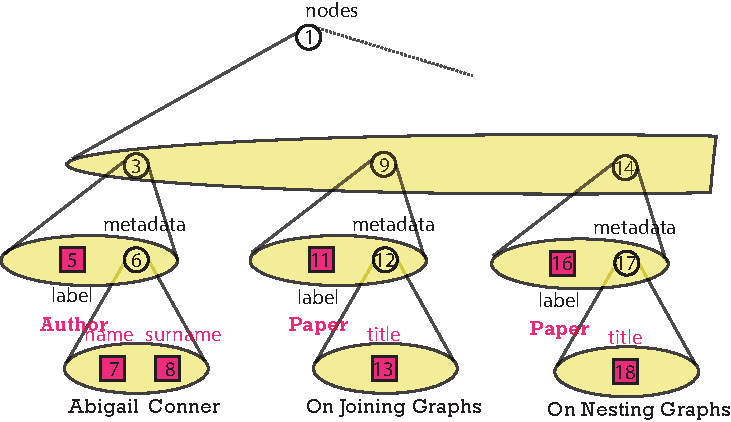
\includegraphics[scale=0.8]{fig/05language/10rearranged_input.pdf}
	\subcaption{Rephrasing the data input for a bibliographical network represented in Figure \vref{subfig:transformationandmatch}.}
	\label{fig:nestingexamples}
\end{minipage}
\begin{minipage}[t]{0.9\textwidth}
	\centering
	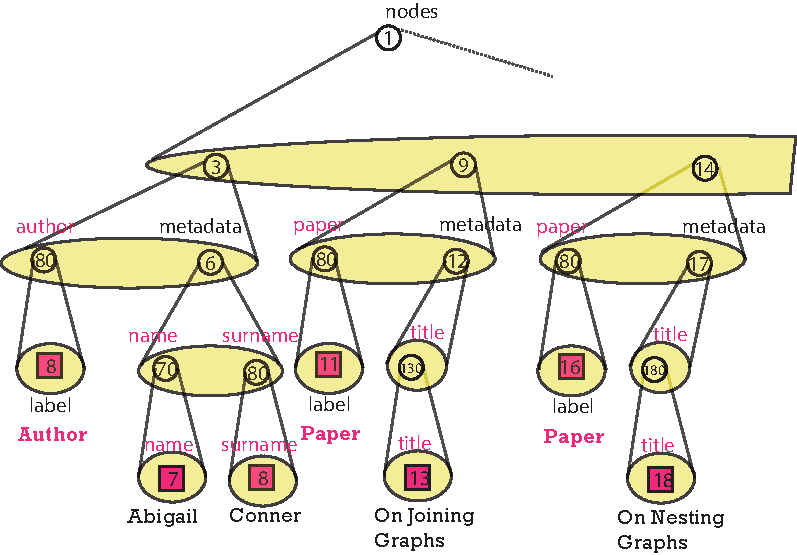
\includegraphics[scale=0.8]{fig/05language/11preserving_aggregation.pdf}
	\subcaption{${\alpha_2}_{GF_1,(k,s)\mapsto [k], (k,s)\mapsto \emptyset, (k,s)\mapsto[[k,\, s]]}^{\texttt{\color{RoyalBlue}tt}}(n)$}
	\label{fig:firstexample}
\end{minipage}
\begin{minipage}[t]{0.9\textwidth}
	\centering
	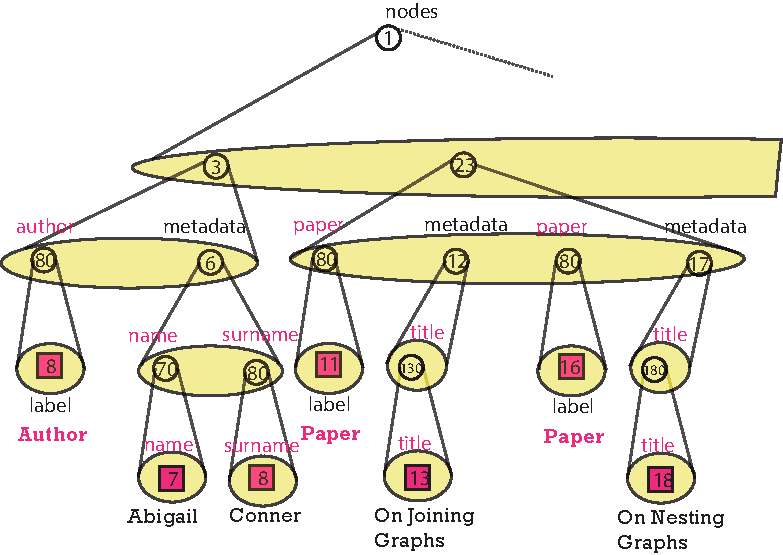
\includegraphics[scale=0.8]{fig/05language/12_intermediate_aggregation.pdf}
	\subcaption{$\texttt{map}_{x\mapsto \ell(x)\backslash{\hstr{\alpha}},\xi,\phi}(\gamma_{GF_2}^{\texttt{\color{RoyalBlue}tt}}({\alpha_2}_{GF_1,(k,s)\mapsto [k,\hstr{\alpha}], (k,s)\mapsto \emptyset, (k,s)\mapsto[[k,\, s]]}^{\texttt{\color{RoyalBlue}tt}}(n)))$}
	\label{fig:secondexample}
\end{minipage}
\caption{Representing different possible results from the application of the general nesting definition. \textit{(cont.)}}
\label{fig:nestingoperations}
\end{figure}

\begin{example}[label=ex:aggregations]
In Example \vref{ex:examplegraphdata} we addressed the problem of extracting the schema from a JSON representation of a graph. As we previously outlined, we could choose to use an aggregation where each matched component via a class $k$ is nested within an object $o$ via $k$, and that $k$ is used as a label for the object that will contain such data. Therefore, the desired result can be achieved via the following application of the $\alpha_2$ aggregator:
\[{\alpha_2}_{GF_1,(k,s)\mapsto [k], (k,s)\mapsto f(s), (k,s)\mapsto[[k,\, s]]}^{\texttt{\color{RoyalBlue}tt}}(n)\]
At this point we want to aggregate each object by its associated label; if the object is a \mstr{label} object, we want to return the value associated to it designign the containing object's label; if the object ha associated to a non relevant label w.r.t. the schema extraction process (e.g. \mstr{metadata}), a set containing the concatenation of the $GF$ classes of all the concatenating object is returned; in all the other cases, no nesting is performed. the following clustering operation describes the desired result:
\begin{equation}
\label{eq:GF1}
GF_1(\_, \_, o)=\begin{cases}
\emptyset & \mstr{metadata}\in\ell(o)\vee P(o)\\
\xi(o) & \mstr{label}\in\ell(o)\\
%\xi(o') &  \min_n (o'\in\varphi^n(o) \wedge \ell(o')=\mstr{label})\\
%\{\bigodot GF(\varphi(o))\} & \mstr{metadata}\in\ell(o)\\%\vee \exists o'\in\varphi(o). GF_1(o')\neq\emptyset\\
\ell(o) & \ell(o)\neq \emptyset\\
\emptyset & \textup{oth.}\\
\end{cases}
\end{equation}
where the underscores remark the ignored arguments.  $P$ is a predicate avoiding to aggregate the elements that are represented only once within the hierarchy and appear at the coarsest levels of it; such predicate is defined as follows:
\[P(x)=(\ell(x)=\emptyset\vee (\neg\exists o'\in\varphi^*(o.n). o'\neq x\wedge \ell(o')=\ell(x)))\wedge(\forall o'\in\varphi^*(o.n).x\in\varphi^+(o')\Rightarrow P(o'))\]
The result of the application of such aggregation to the nested structure represented in Figure \ref{fig:nestingexamples} is provided in Figure \ref{fig:firstexample}: this operation preserves all the original data within each aggregated element but, at the same time, increases the amount of generated data. As a consequence, this solution could potentially increase the time required to visit the data structure that may occur at subsequent steps. Therefore, a different approach preserving the GSM height in spite of the representation of the original information is required.
\end{example}

\phparagraph{Grouping ($\gamma$)}
The grouping operation for semistructured data  was originally presented in \cite{Magnani06}, where  $\oplus_f$ is simply defined as the $n$-ary union of all the matched objects, thus allowing to integrate each similar component into one single representation. The desired operation can be described as follows: \index{GSQL!$\gamma$}
\begin{equation}\label{eq:grouping}
\gamma_{GF}^{\textbf{keep}}(n)=\nu^{\textbf{keep}}_{GF,\genp,(\alpha,k,\tilde{o}_{c},s)\mapsto \texttt{elect}_{o}\left(\bigcup^{\tilde{o}_c}_{i\in s}\texttt{elect}_i(\alpha)\right)}(n)
\end{equation}
\begin{example}[continues=ex:aggregations,label=ex:aggregations2]
Figure \ref{fig:secondexample} shows an example of grouping. In this case we want to aggregate even the elements that were not previously inserted within a cluster. Therefore, we change the $\alpha_2$ by marking with $\hstr{\alpha}$ the elements matched by $GF_1$.
%\begin{equation}
%\widetilde{GF_1}(\_,\_,o)=\begin{cases}
%\emptyset & P(o)\\
%\xi(o)\cup\{\hstr{\alpha}\} & \mstr{label}\in\ell(o)\\
%\{\bigodot GF(\varphi(o))\}\cup\{\hstr{\alpha}\} & \mstr{metadata}\in\ell(o)\\
%\ell(o)\cup\{\hstr{\alpha}\} & \ell(o)\neq \emptyset\\
%\emptyset & \textup{oth.}\\
%\end{cases}
%\end{equation}
Last, the following $GF$ function for $\gamma$ is provided:
%\[GF_2(\_,\_,o)=\begin{cases}
%\ell(o)\backslash\{\hstr{\alpha}\} & \hstr{\alpha}\in\ell(o)\\
%\ell(o) & (P(o)\wedge \ell(o)\neq\emptyset ) \vee \exists o'\in\varphi^+(o).\hstr{\alpha}\in\ell(o') \\
%\xi(\min S) & P(o)\wedge (S= \argmin_{\tsub{o''\in \varphi^*(o.n)\cap\varphi^+(o)\\ \mstr{label}\in\ell(o'')}}rh(o,o'') \wedge S\neq\emptyset)\\
%\emptyset & \textup{oth.}\\
%\end{cases}\]
\[GF_2(\_,\_,o)=\begin{cases}
\ell(o)\backslash\{\hstr{\alpha}\} & \hstr{\alpha}\in\ell(o)\\
\ell(o) & \ell(o)\neq\emptyset \wedge \exists o'\in\varphi^+(o). GF_2(\_,\_,o')\neq\emptyset \\
\bigodot_{o'\in\varphi(o)}GF_2(\_,\_,o') & \ell(o)=\emptyset\\
\emptyset & \textup{oth.}\\
\end{cases}\]
where $\bigodot$ is the string concatenation function over set of strings.
As we can see, this operation does not structurally propagate the aggregation within all the containment levels, but it only aggregates the data at the first nesting level available. In order to propagate the nesting in depth, we must iterate the same operation until all the similar components are structurally aggregated together. Therefore, it is now relevant why the \texttt{fold} construct is relevant for our algebra.
\end{example}


\phparagraph{Abstraction ($\alpha_1$)}\label{abstractionAlpha1}

Let us now discuss on how to achieve the $\alpha$ schema extraction operator over our nested data representation. In the previous chapter we mentioned that, within this thesis, we are going to work exclusively on nesting-loop free GSMs: this constraint allows a definition of structural length of a GSM. Given that the structured aggregation must be further propagated towards the leaves after each iteration, we can consider the GSM's height as an upper bound to the number of iterations required to propagate the aggregations as expected. Therefore, we may first perform an $\alpha_2$ aggregation and, after that, we can recursively group by the former labels. Such operator may be defined as follows:



\begin{definition}[Structural Aggregation]
	\index{GSQL!$\alpha_1$}
	Given an equivalence relation $SF$ to be tested among the objects within each containment $\phi(o,p)$, the structural aggregation propagates the aggregation result to all the underlying data structures by marking them with a $\hstr{\alpha}$ label. This operator is then defined as follows:
	\[{\alpha_1}_{SF}^{\textbf{keep}}(n)=\gamma_{GF_2}^{\textbf{keep}}(\alpha)(\texttt{fold}_{\Set{i\in \nat|0<i< h(n)},x\mapsto\alpha\mapsto \gamma_{GF_2}^{{\color{RoyalBlue}\texttt{tt}}}(\alpha)}({\alpha_2}_{SF,(k,s)\mapsto [k,\hstr{\alpha}], (k,s)\mapsto \emptyset, (k,s)\mapsto[[k,\, s]]}^{{\color{RoyalBlue}\texttt{tt}}}(n)))\]
\end{definition}

\begin{figure}[!t]
	\ContinuedFloat
	\centering
	\begin{minipage}[t]{0.5\textwidth}
		\centering
		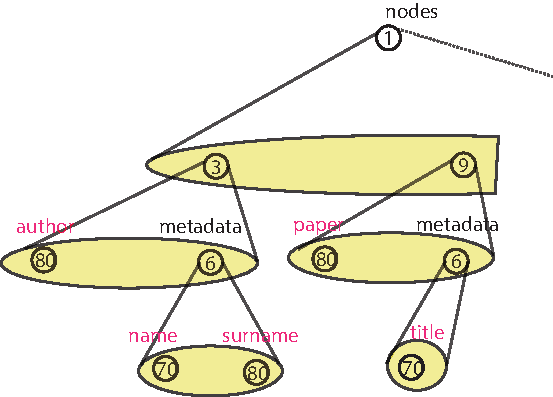
\includegraphics[scale=0.8]{fig/05language/13actual_schema.pdf}
		\subcaption{$\texttt{map}_{x\mapsto \ell(x)\backslash{\hstr{\alpha}},\xi,\phi}({\alpha_1}_{GF_1}^{{\color{RoyalBlue}\texttt{ff}}}(n))$}
		\label{fig:finalexample}
	\end{minipage}
	\caption{Representing different possible results from the application of the general nesting definition.}
\end{figure}
\begin{example}[continues=ex:aggregations2]
Figure \vref{fig:finalexample} provides the desired solution allowing to implement the schema extraction operation outlined in Example \vref{ex:examplegraphdata} for the data integration scenario.
In order to met the requirements of the former definition, $GF_1$ presented in Equation \vref{eq:GF1} is used for the first aggregation step, while the remaining ones are performed via the following function applied to has to be extended in order to mark the elements that must be structurally aggregated.
\end{example}

After performing this operation, we can now aggregate the left out elements, thus allowing to implement the relational group over overlapping classes.

\begin{definition}[Multi Group-By]
	\index{$\Gamma$!for GSQL|see {GSQL}}\index{GSQL!$\Gamma$}
Given an equivalence relation $SF$ to be tested among the objects within each containment $\phi(o,p)$ and an aggregation function expressed by the three functions $f_L,f_E,f_C$ to be applied over the remaining non-aggregated objects via $SF$, the \textbf{multi group by} over a GSM $n$ is defined as follows:
	\[\Gamma_{SF}^{f_L,f_E,f_C}(n)={\alpha_2}_{(o,p,o')\mapsto {\color{webgreen}\textup{``}\alpha\textup{''}}\notin\ell(o')?{\color{webgreen}\textup{``}\alpha\textup{''}}:\emptyset}^{\texttt{\color{RoyalBlue}tt},f_L,f_E,f_C}({\alpha_1}_{SF}^{{\color{RoyalBlue}\texttt{tt}}}(n))\]
\end{definition}



\phparagraph{$\otimes\theta$-Product}
\index{product!$\otimes_\theta$!for GSQL|see {GSQL}}\index{GSQL!$\otimes_\theta$ product}
\label{def:otimesthetaList} 
Given that $\otimes\theta$-products take two GSMs as an input and provide one single GSM, we must 
%In this scenario we must suppose that we 
preliminarily merge the two operands $n$ and $n'$ via a disjoint union $\texttt{disjoint}^{\omega_c}(n, n')$. Consequently, the input GSM's reference objects are considered as multiple labelled sets and, therefore, the final join operation shall be performed among all the collections appearing in the left and right  operand. In particular, for each collection $\phi(\omega_c,[1,p'])$ and $\phi(\omega_c,[2,p''])$ respectively coming from the first and second operand, we want to return a new collection $\phi(\omega_{c+1},p'p'')$ containing the result of the $\otimes_\theta$ product of the contained objects. As a final result, a \texttt{create} predisposing the $p'p''$ collection has to be performed immediately after the disjoint union.%, and that $GF$ contains the reference to the binary predicate $\theta$ and is defined as follows:

The clustering function $GF$ shall create a distinct cluster for each pair of matching objects $x$ and $y$, respectively contained in the collections $\phi(\omega_c,p')$ and $\phi(\omega_c,p'')$, and then associates each object to the pairs $\texttt{bin}(p')\texttt{bin}(p'')xy$. Such set of elements will be used in the clustering function (Equation \ref{positive-subnum}) and can be defined as follows:
\[\begin{split}
JS_{\omega_c,p',p''}^\textbf{c}(x)=&\{(\texttt{bin}(p')\cdot\texttt{0}\cdot \texttt{bin}(p'')xy)_{c+1}|\theta(x,y),x\in\phi(\omega_{c},[1,p']),y\in\phi(\omega_{c},[2,p'']) \}\\
	&\cup\{(\texttt{bin}(p')\cdot\texttt{0}\cdot\texttt{bin}(p'')yx)_{c+1}|\theta(y,x),x\in\phi(\omega_{c},[2,p'']),y\in\phi(\omega_{c},[1,p']) \}
\end{split}\]
On the other hand, each $[1,p]$ and $[2,p'']$ collection contained in $\texttt{disjoint}^\omega(n',n'')$ must be empty (Equation \ref{GFotherwise}) while all the remaining objects' containment should be kept unaltered (Equation \ref{negative-subnum}).The whole definition of $GF$ is defined as follows:
\begin{subnumcases}{GF_{\theta}(o,p,x)=}
JS_{\omega_c,p',p''}^\textbf{c}(x) & $o=\omega_{c+1},p=p'p''.[1,p'],[2,p'']\in\dom(\phi(\omega_c))$ \label{positive-subnum}\\
\bot & $o\neq\omega_{c+1}$ \label{negative-subnum}\\
\emptyset & oth.\label{GFotherwise}
\end{subnumcases}
This definition is then involved in two different roles: first, \textit{(\textbf{i})} $GF_\theta$ is used in Equation \vref{eq:ce} to generate the pairs $(o,p'p'',\texttt{bin}(p')\cdot\texttt{0}\cdot\texttt{bin}(p'')xy)$, so that the aggregation function $J_\otimes$ used for $\oplus_f$ is able to generate a new object by $\otimes$-concatenating the two  objects  $u$ and $v$ matching with predicate $\theta$ for containments $b_1$ and $b_2$:
\[J_\otimes(\alpha,\texttt{bin}(p')\cdot\texttt{0}\cdot\texttt{bin}(p'')xy,\omega,s)=\texttt{elect}_{\omega}\left(\bigotimes^{\texttt{bin}(p')\cdot\texttt{0}\cdot\texttt{bin}(p'')xy}_{u\in s}\texttt{elect}_u(\alpha)\right)\]
where $\otimes$ is a generic aggregation operation for each element $u$ appearing in the cluster for the elements matching the cluster label $\texttt{bin}(p')\cdot\texttt{0}\cdot\texttt{bin}(p'')xy$ that is going to be used for an object identifier for the previously-aggregated element. Then, the operators re-set $\omega$ as a reference object over which perform the remaining operations. 
For the relational join purposes, we can choose the previously-introduced  concatenation operator $\oplus$ as $\otimes$ for combining the matched objects. 
\medskip

Last, \textit{(\textbf{ii})} the $JS$ function within the $GF_\theta$ classifier is used in cooperation with $\genp'$ to define which are the resulting containments, directly generated by $GF_\theta$ as a result of the $\otimes\theta$-product operator, and which are the elements that are not involved by the $\otimes\theta$-product operation ($o_{\tilde{c}}\neq \omega$); while in the first case the result of the $\otimes_\theta$ combination shall be returned for each matched pair of objects (Equation \ref{vargammafst}), for the other cases where the resulting reference object is not involved and hence the involved \texttt{map} must neither change nor update their containments must be preserved (Equation \ref{vargammasecond}). 
\begin{subnumcases}{\genp'(o_{\tilde{c}},k,o,p)=}
\phi(o,p) & $k = \bot$ \label{vargammafst}\\
k &  oth.\label{vargammasecond}
\end{subnumcases}
Consequently, the binary $\otimes\theta$-product operation can be defined as follows\index{product, $\otimes_\theta$!for GSM}:
\[n \otimes_{JS,\theta} n'=\nu_{GF_\theta,\genp',J_\otimes}^{\texttt{\color{RoyalBlue}ff}}(\texttt{create}^{\omega_{c+1}}_{\ell(\omega_c),\xi(\omega_c),\oplus_{\tsub{$[1,p']$,\\ $[2,p'']\in\dom(\phi(\omega_c))$}}\;[[p'p'', \phi(\omega_c,[1,p'])\cup \phi(\omega_c,[2,p''])]]\;}(\texttt{disjoint}^{\omega_c}(n,n')))\]
Consequently, by replacing $\otimes$ with $\oplus$ we achieve and by constraining $\theta$ to check that all the elements contained by the to-be-merged elements and having the same $\ell$ label must show the same $\xi$ values, we have the implementation of the join operator, thus the following expression provides the join definition alongside the definition of the restriction for $\theta$:
\[n \bowtie_\theta n'\eqdef n \oplus_{JS^c,\substack{(x,y)\mapsto\theta(x,y)\wedge \forall e\in\dom(\phi(x))\cap\dom(\phi(y)).\\\forall x'\in\phi(x,e).\forall y'\in \phi(y,e).\\ \ell(x')\cap\ell(y')\neq \emptyset\Rightarrow \xi(x')=\xi(y')=\emptyset \vee \xi(x')\cap\xi(y')\neq\emptyset. }} n' \]
